\chapter{Dataset}\label{sec:dataset}

For the purposes of this project, we used a dataset that allows us to associate a CT scan and an X-ray of the same patient acquired with a relatively short time gap; this let us to be reasonably confident about the correlation of information present in these two exams.
Comparing our dataset to that used by \citeauthor{zhang2023distilling} in \cite{zhang2023distilling} that develop a similar KD approach, we can note that our data association is more conservative and we suppose should be more reliable: their pairing of data from different modalities is performed matching samples belonging to the same class, whereas we are pairing data from the same patient.

In particular, our dataset has been provided by \emph{Città della Salute e della Scienza di Torino} hospital and is composed by 491 paired frontal CXRs and relative CT scans of the same patients, labelled by experts with the CAC score.
Beside the paired samples, we exploited also 112 additional CXRs without their respective CT scans, that we use to validate our results during the testing phase.

The paired scans has been acquired at 39 days apart on average, with values ranging from both analysis performed on the same day up to about 3 years, median value is 12 days.
Time gap between exams is important for the reliability of labelling considering that CAC scoring is performed on CTs.
Based on the order in which the tests are performed and on the class the patient belongs to, we can divide the possible cases into four possible scenario:
\begin{itemize}
    \item CT before CXR on negative patient: if long time occurs between the two exams the patient could turn to positive in the meantime and classification on CXR is compromised.
    \item CT before CXR on positive patient: since no known pharmacological methods can lead to CAC regression \cite{Czaja-Ziolkowska2022-pd} we are sure that when the CXR is performed the CAC is still positive and its value may only be greater or equal than before. 
    \item CT after CXR on negative patient: for the same reason as before, the patient was certainly already negative when CXR was performed.
    \item CT after CXR on positive patient: in this case it is possible that the patient was negative when CXR was performed and became positive during the time elapsed between exams.
\end{itemize}
However, the time gap between our paired samples is generally short enough to give us a good confidence about reliability of the classification, with low probability that class of the patient can change between the two exams.

In the following section we describe the image we have at our disposal, whereas in \ref{sec:dataset_distribution} we perform an accurate statistical analysis of our dataset, in order to have clear in mind what kind of data we are using.


\section{Image types: CT scans and CXR}

\subsection{CT Scans}

The 491 CT scans has been acquired by 9 different devices, using different protocols, and focusing on different portion of the body.
Indeed, some of them focus on the cardiac area only, with a very high resolution, some have a slightly larger field of view, including the whole body width, and a lower resolution.
Slice thickness is between 0.6mm and 3mm with an average of 1.3mm and a median and mode of 1.25mm.
All scans are composed by a variable number of slices between 123 and 1100 of the same size of $512 \times 512$ voxels, with only 2 exceptions that are $768 \times 768$.
Despite their differences, they are all suitable for CAC scoring performed by experts, and we assume that a properly trained NN could effectively perform CAC detection on them.
Some examples of different types of CT scans available in our dataset are depicted in figure \ref{fig:ct_example}.

\begin{figure}
    \centering
    \begin{subfigure}[b]{0.3\textwidth}
        \resizebox{\textwidth}{!}{ 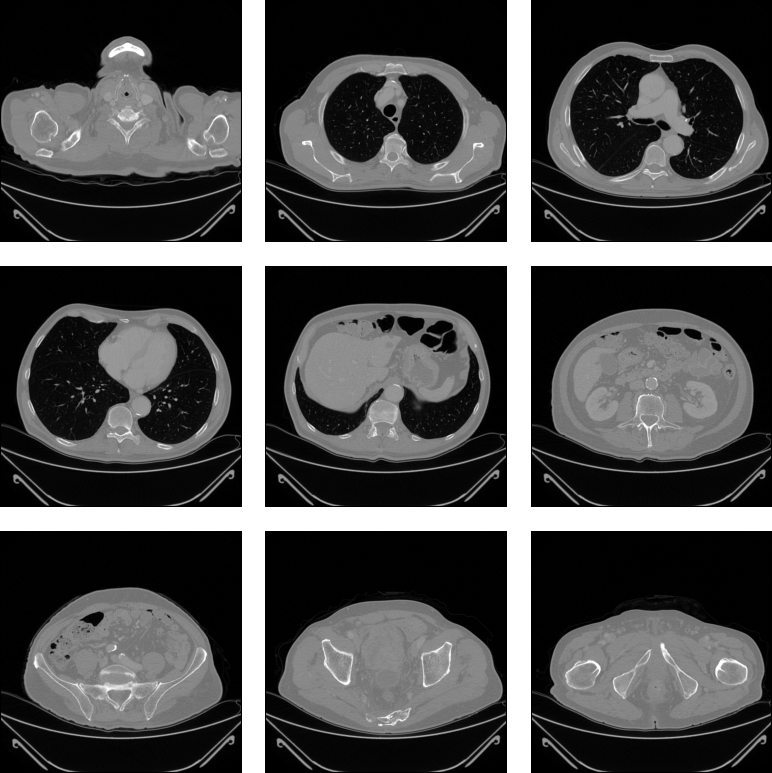
\includegraphics{ct_example_large} }
        \caption{}
        \label{subfig:ct_example_large}
    \end{subfigure}\hspace{1em}
    \begin{subfigure}[b]{0.3\textwidth}
        \resizebox{\textwidth}{!}{ 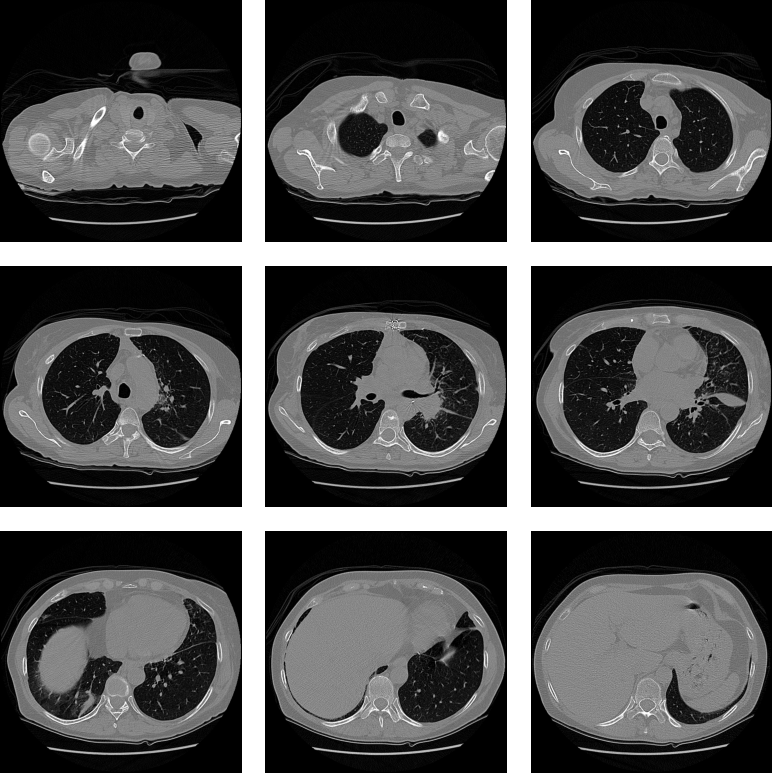
\includegraphics{ct_example_medium} }
        \caption{}
        \label{subfig:ct_example_medium}
    \end{subfigure}\hspace{1em}
    \begin{subfigure}[b]{0.3\textwidth}
        \resizebox{\textwidth}{!}{ 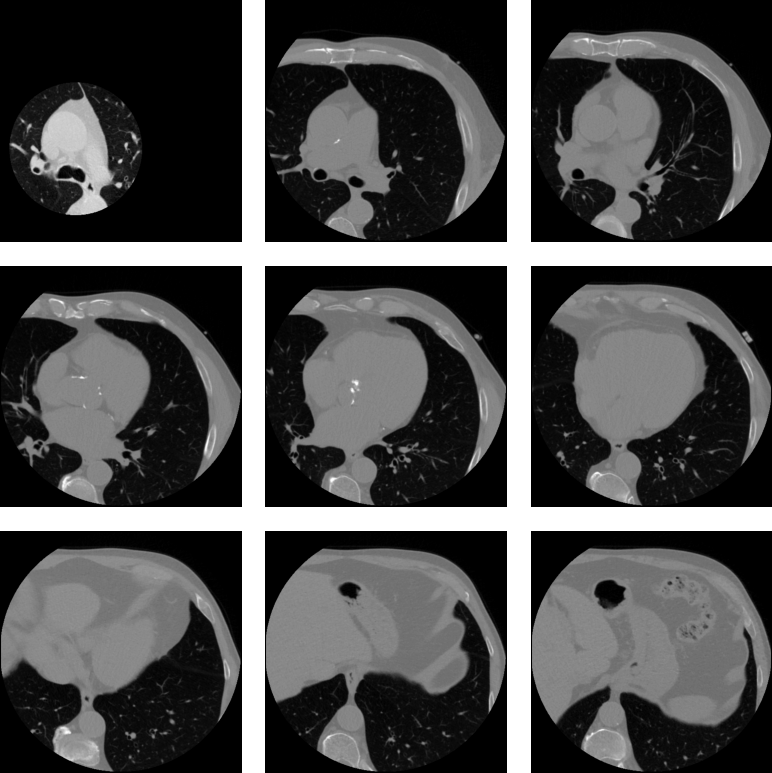
\includegraphics{ct_example_small} }
        \caption{}
        \label{subfig:ct_example_small}
    \end{subfigure}
    
    \caption{Some slices in axial projection at increasing depths of 3 CT scans acquired using different protocols and different fields of view. Images from our dataset.}
    \label{fig:ct_example}
\end{figure}


\subsection{CXR}

Differently from CTs, the 603 CXRs have been acquired by more than 20 different devices in different projections, 408 of them are marked as posteroanterior views; this projection is preferable since the heart is generally clearly visible on it.
The remaining images are anteroposterior, where the image is often blurred and heart shape is deformed.
For 44 patients also a lateral CXR is available, but those images are not considered for this work since visibility of the heart is limited and the number of samples is very low.
Main differences between the three possible CXR projections can be observed in some examples depicted in figure \ref{fig:cxr_example}.
The size of the images are varying, from a minimum of $1733\times1715$ to a maximum of $4020\times4892$, presented in different proportions.

This dataset extends the one used by \cite{iodice_2022}, including all the CXRs used in that work.

\begin{figure}
    \centering
    \begin{subfigure}[b]{0.3\textwidth}
        \resizebox{\textwidth}{!}{ 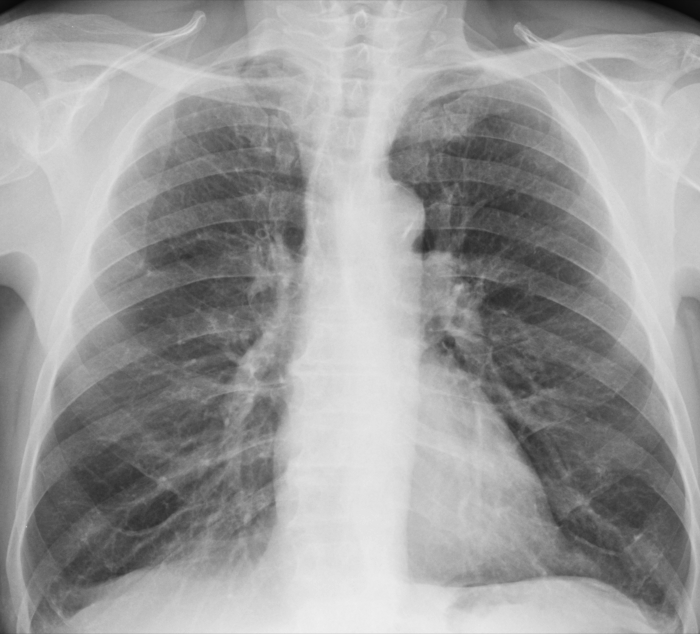
\includegraphics{cxr_example_pa} }
        \caption{}
        \label{subfig:cxr_example_pa}
    \end{subfigure}\hspace{1em}
    \begin{subfigure}[b]{0.3\textwidth}
        \resizebox{\textwidth}{!}{ 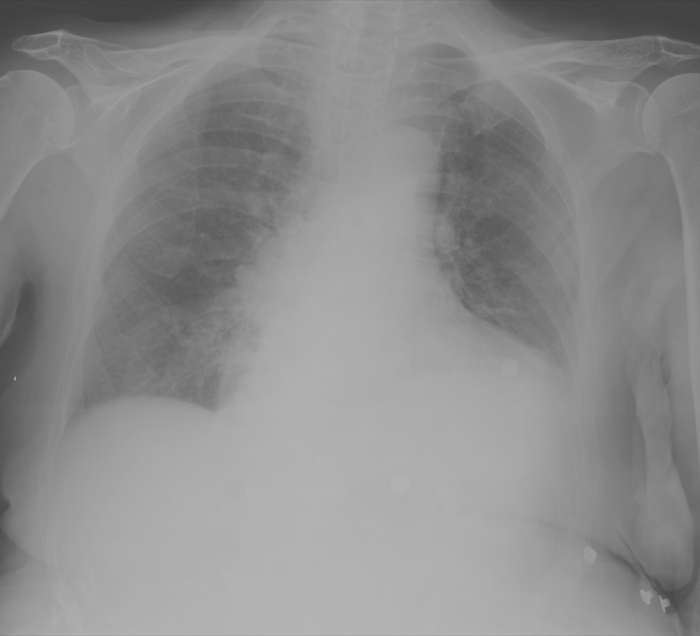
\includegraphics{cxr_example_ap} }
        \caption{}
        \label{subfig:cxr_example_ap}
    \end{subfigure}\hspace{1em}
    \begin{subfigure}[b]{0.3\textwidth}
        \resizebox{\textwidth}{!}{ 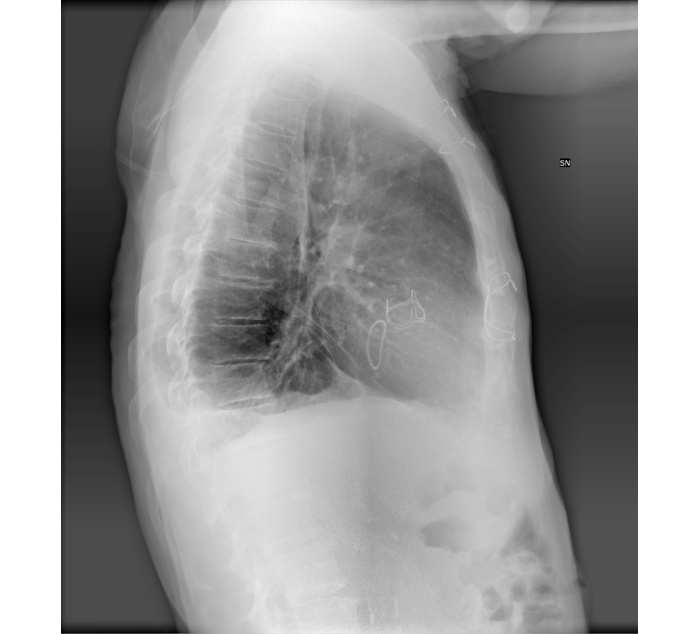
\includegraphics{cxr_example_lat} }
        \caption{}
        \label{subfig:cxr_example_lat}
    \end{subfigure}
    
    \caption{Examples of (a) posteroanterior, (b) anteroposterior and (c) lateral X-rays.
             Images from our dataset.}
    \label{fig:cxr_example}
\end{figure}


\section{Statistical analysis of the clinical data}\label{sec:dataset_distribution}

In this section we analyze the clinical data (i.e. age, gender, CAC distribution) associated to our dataset, that is composed by patients aged between 3 and 93 years, with an average age of 62 years.
Distribution of patients by age is depicted in figure \ref{subfig:dataset_patients_by_age}; the most represented class is that of people in their sixties and over 60\% of the dataset is composed by people over this age.
From figure \ref{subfig:dataset_cac_avg_by_age}, we can see that all patients below 30 years are negatives while people above 60 years have, on average, a CAC score greater than 1000.
Generally we can see that CAC score increases with age, with the only exception of the class of people above age of 90 that has, however, very few samples.

Figure \ref{subfig:dataset_patients_by_cac} shows distribution of patients by CAC score grouped by risk categories of table \ref{tab:agatston-risk}, with 39\% of patients in the very low risk category, i.e. negative class in our task with no calcium detected, and 61\% with a CAC score greater that zero; of them the majority is in the very high risk category.
The low, intermediate and high risk classes are less represented in our dataset and those likely contain patients that are presumably harder to classify; this is an additional complication to solve our classification task, since indeed more samples of those classes could be helpful to train a better classifier.
The dataset is also biased towards male gender, that represents 60\% of patients,  67\% of them have positive value of CAC, against 51\% of positives in the female subset, as shown on figure \ref{subfig:dataset_cac_by_gender}.

An overall summary of class distribution across gender and age is shown in table \ref{tab:pos_neg_distribution}.
Distribution of our dataset is consistent with other studies, showing that the likelihood of developing CAC increases with age and is related to gender \cite{Czaja-Ziolkowska2022-pd}.

\begin{figure}
    \centering
    \begin{subfigure}[b]{0.45\textwidth}
        \resizebox{\textwidth}{\textwidth}{ \begin{tikzpicture}
    \begin{axis}[
        name=age_plot,height=9cm,width=9cm,
        % title={Age distribution},
        ybar,
        ymin=0,ylabel={Patients},
        xmin=0,xmax=100,xlabel={Age} 
    ]
        \addplot +[
            hist={
                bins=10,
                data min=0,
                data max=100
            }   
        ] table [y index=0] {data/age.csv};
    \end{axis}
\end{tikzpicture}
 }
        \caption{}
        \label{subfig:dataset_patients_by_age}
        \vspace*{3em}
    \end{subfigure}
    \begin{subfigure}[b]{0.45\textwidth}
        \resizebox{\textwidth}{\textwidth}{ 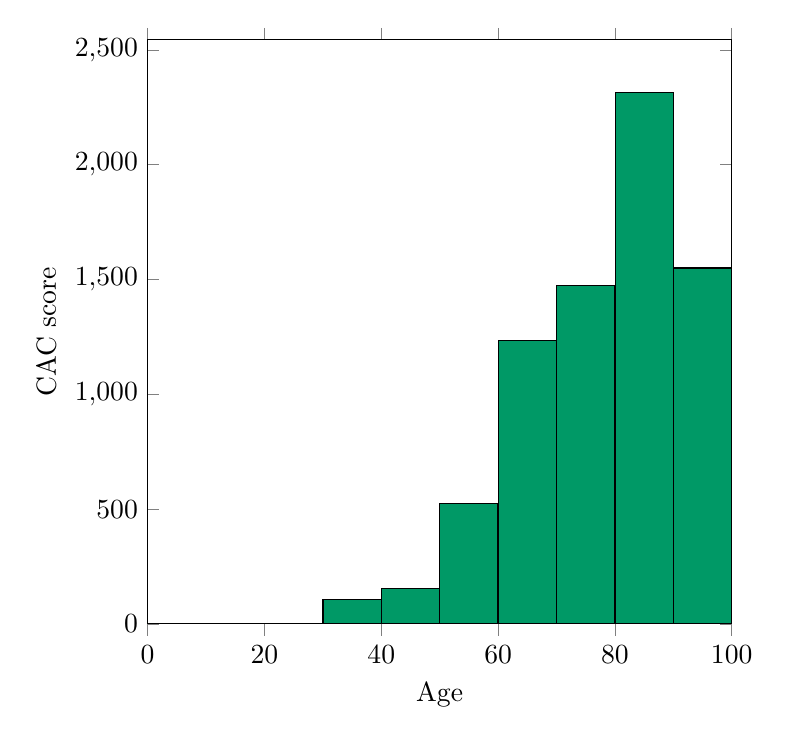
\begin{tikzpicture}
    \begin{axis}[
        name=cac_avg_by_age,height=9cm,width=9cm,
        ybar,
        ymin=0,ylabel={CAC score},
        xmin=0,xmax=100,xlabel={Age},
        bar width=21pt,
    ]
        \addplot[fill=green!60!blue] coordinates {
            (5,0)
            (15,0)
            (25,0)
            (35,107)
            (45,155)
            (55,525)
            (65,1234)
            (75,1474)
            (85,2313)
            (95,1550)
        };
    \end{axis}
\end{tikzpicture}
 }
        \caption{}
        \label{subfig:dataset_cac_avg_by_age}
        \vspace*{3em}
    \end{subfigure}

    \begin{subfigure}[b]{0.45\textwidth}
        \resizebox{\textwidth}{\textwidth}{ \begin{tikzpicture}
    \begin{axis}[
        name=cac_plot,at={($(age_plot.east)+(2cm,0)$)},anchor=west,height=9cm,width=9cm,
        % title={CAC score distribution},
        ybar,
        symbolic x coords={0, 1-10, 11-100, 101-400, >400},
        ymin=0,ylabel={Patients},
        xmin=0,xtick=data,xlabel={CAC score},
        bar width=30pt,
        enlarge x limits=0.1,
        % nodes near coords={\pgfmathprintnumber\pgfplotspointmeta} % put value on bar top
    ]
        \addplot[fill=orange!70] coordinates {
            (0,235)
            (1-10,10)
            (11-100,55)
            (101-400,64)
            (>400,239)
        };
    \end{axis}
\end{tikzpicture}
 }
        \caption{}
        \label{subfig:dataset_patients_by_cac}
    \end{subfigure}
    \begin{subfigure}[b]{0.45\textwidth}
        \resizebox{\textwidth}{\textwidth}{ 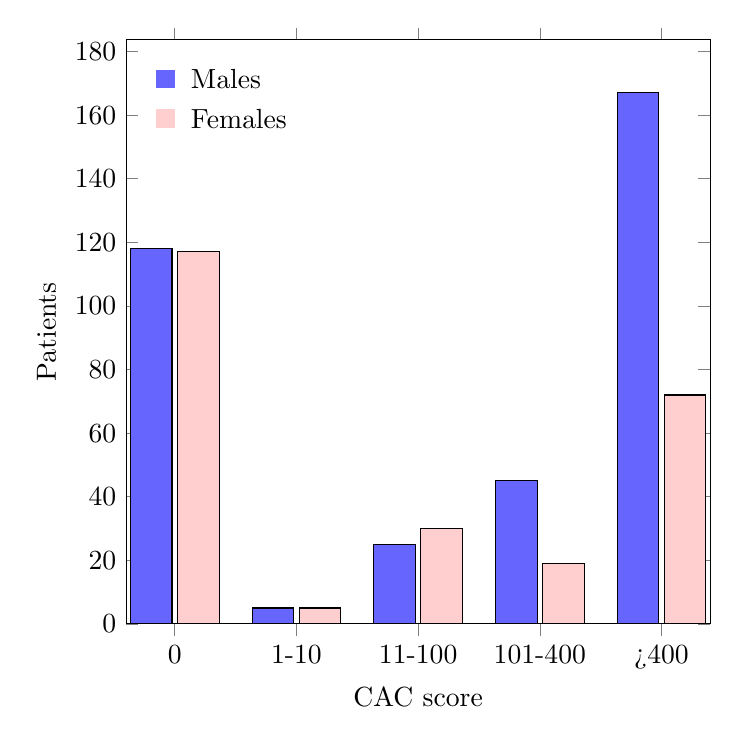
\begin{tikzpicture}
    \begin{axis}[
        name=cac_by_gender,height=9cm,width=9cm,
        % title={CAC score by gender distribution},
        ybar,
        symbolic x coords={0, 1-10, 11-100, 101-400, >400},
        ymin=0,ylabel={Patients},
        xmin=0,xtick=data,xlabel={CAC score},
        bar width=15pt,
        enlarge x limits=0.1,
        % nodes near coords={\pgfmathprintnumber\pgfplotspointmeta} % put value on bar top
    ]
        \addplot[fill=blue!60] coordinates {
            (0,118)
            (1-10,5)
            (11-100,25)
            (101-400,45)
            (>400,167)
        };
        \addplot[fill=pink!75] coordinates {
            (0,117)
            (1-10,5)
            (11-100,30)
            (101-400,19)
            (>400,72)
        };
    \end{axis}
    \node[fill=blue!60,xshift=0.5cm,yshift=-0.5cm] at (cac_by_gender.north west) (male) {};
    \node[right of=male,anchor=west,xshift=-0.8cm] {Males};
    \node[fill=pink!75,below of=male,yshift=0.5cm] (female) {};
    \node[right of=female,anchor=west,xshift=-0.8cm] {Females};
\end{tikzpicture}
 }
        \caption{}
        \label{subfig:dataset_cac_by_gender}
    \end{subfigure}\hspace{1em}

    \caption{(a) Dataset distribution of patients by age, (b) CAC average by age, (c) patients by CAC score grouped by risk category, (d) CAC distribution by gender and risk category.}
    \label{fig:dataset_distribution}
\end{figure}

\begin{table}
    \centering
    \begin{tabular}{|l|r c|r c|c|}
        \hline
        & \multicolumn{2}{c|}{\textbf{Negatives}} & \multicolumn{2}{c|}{\textbf{Positives}} & \textbf{TOTAL} \\
        \hline
        Male    & 118 & (32,8\%) & 242 & (67,2\%) & 360 \\
        Female  & 117 & (48,1\%) & 126 & (51,9\%) & 243 \\
        \hline
        Age 0-9   &   1 &  (100\%) &   0 &    (0\%) &   1 \\
        Age 10-19 &  13 &  (100\%) &   0 &    (0\%) &  13 \\
        Age 20-29 &  28 &  (100\%) &   0 &    (0\%) &  28 \\
        Age 30-39 &  28 & (96,6\%) &   1 &  (3,4\%) &  29 \\
        Age 40-49 &  47 & (79,7\%) &  12 & (20,3\%) &  59 \\
        Age 50-59 &  54 & (52,9\%) &  48 & (47,1\%) & 102 \\
        Age 60-69 &  42 & (29,0\%) & 103 & (71,0\%) & 145 \\
        Age 70-79 &  13 &  (9,8\%) & 120 & (90,2\%) & 133 \\
        Age 80-89 &   8 & (10,0\%) &  72 & (90,0\%) &  80 \\
        Age 90+   &   1 &  (7,7\%) &  12 & (92,3\%) &  13 \\
        \hline
        \hline
        Training set   & 164 & (40.3\%) & 243 & (59.7\%) &    407 \\
        Test set (CT)  &  32 & (38.1\%) &  52 & (61.9\%) &     84 \\
        Test set (CXR) &  71 & (36.2\%) & 125 & (63.8\%) & 84+112 \\
        \hline
        \hline
        ALL       & 235 & (39,0\%) & 368 & (61,0\%) & 603 \\
        \hline
    \end{tabular}
    \caption{Distribution of data between positives and negatives classes}
    \label{tab:pos_neg_distribution}
\end{table}

Throughout this work, the dataset has been split in two parts to compose a training set and a test set with approximately same class distribution.
From the entire set of patients with both a CXR and a CT scan, we removed randomly 84 samples to compose the test set, the remaining have been used as the training set.
Furthermore, as mentioned at the beginning of this chapter, all 112 CXRs that do not have a paired CT scan have been included in the test set of the experiments that use X-ray images as inputs, for a total of 196 samples.
